\documentclass{article}[11pt]
\usepackage[utf8]{inputenc}

\usepackage{subcaption}
\usepackage{caption}

\usepackage{tikz-qtree}

\title{6.035 Semantic Checking and Unoptimized Code Generation}
\author{Hayk Saribekyan, Tsotne Tabidze, Akaki Margvelashvili}
\date{March 2016}


\usepackage{listings,lstautogobble}
\usepackage{xcolor}

\definecolor{RoyalBlue}{cmyk}{1, 0.50, 0, 0}

\lstset{language=Java,
    keywordstyle=\color{RoyalBlue},
    basicstyle=\scriptsize\ttfamily,
    commentstyle=\ttfamily\itshape\color{gray},
    stringstyle=\ttfamily,
    showstringspaces=false,
    breaklines=true,
    % frameround=ffff,
    % frame=single,
    rulecolor=\color{black},
    autogobble=true
}

\begin{document}

\maketitle

\section{Introduction}
In this document we explain the design and implementation of a semantic checker and a generator for unoptimized code for Decaf language, which is a simple C-like language.

The document will first introduce the starting point for doing semantic check. The subsequent sections will describe the general design approaches and implementation details for semantic checking and code generation.

The compiler is implemented in Java.

\section{Background}
The first stages of building a compiler (scanner and parser) are out of the scope of this document. The code for both the scanner and the parser is generated using ANTLRv2. This step involves precisely writing formal language rules of Decaf in ALTLR's meta-language.

\section{Intermediate Representation - Level 1}
After scanning and parsing the program, the compiler needs to build an intermediate representation for the sample program that it can handle more easily. This section will describe how we build the first level intermediate representation (IR-1) from AST. After we have the AST building IR-1 is straightforward.

\subsection{Abstract Syntax Tree Generation}
\label{sec:ast}
Without extra modifications, the output of a parser generated by ANTRL is a concrete syntax tree (CST), which is very hard to manipulate in the later stages of the compiler. CST is needed to resolve ambiguities in the language grammar using semantic rules, such as operator precedence.

We therefore need to convert the CST to abstract syntax tree (AST). We have used options provided by ANTLR, which allow the parser to generate an AST directly. In ANTLR the roots of the AST have to be scanner tokens (e.g. for operators) and \textit{imaginary} tokens (mainly for larger units of the program such as the program itself or blocks). Figure \ref{fig:ast} shows an example of a small code snippet of Decaf and its corresponding AST. Note that the AST does not have any information about parentheses or semicolons in the Decaf language. AST has the "minimal" amount of information needed for correct code generation.

Note the "..." in the AST in Figure \ref{fig:ast}. In order to keep operator precedence in expression, it is needed to have separate nodes for all types of expression (e.g. addition, subtraction, array length, ternary) to have separate node representing it. These are represented by the "..." in the AST.

\begin{figure}
%   \hspace{-1.5cm}
   \begin{subfigure}{0.45\linewidth}
        \begin{lstlisting}[language=C]
        int a;
        void main() {
            int b;
            a += b;
        }
        \end{lstlisting}
   \end{subfigure}
   \hspace{-2.5cm}
   \begin{subfigure}{0.45\linewidth}
        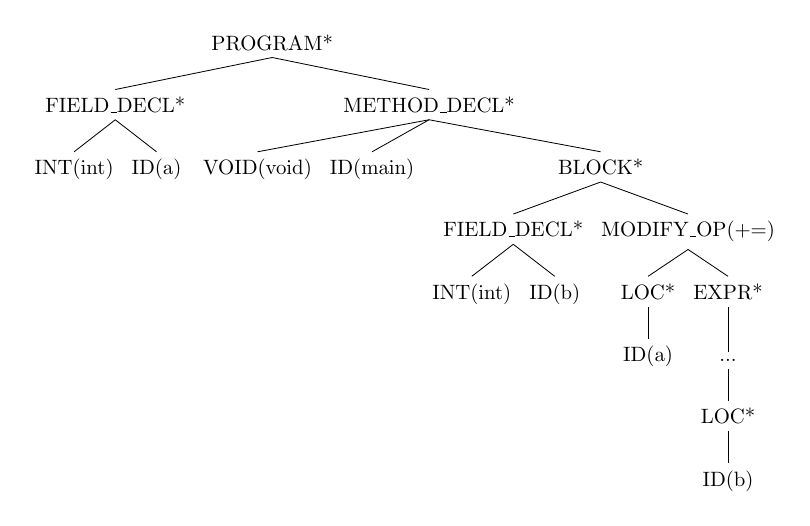
\begin{tikzpicture}[scale=.75]
        \Tree[.PROGRAM* [.FIELD\_DECL* [.INT(int) ] 
                                         [.ID(a) ] ]
                         [.METHOD\_DECL* [.VOID(void) ]
                                          [.ID(main) ]
                                          [.BLOCK* [.FIELD\_DECL* [.INT(int) ]
                                                                    [.ID(b) ] ]
                                                    [.MODIFY\_OP(+=) [.LOC* [.ID(a) ] ]
                                                                     [.EXPR* [.... [.LOC* [.ID(b) ] ] ] ] ] ] ] ]
        \end{tikzpicture}
   \end{subfigure}
   
   \caption{Simple code in Decaf and its corresponding AST. The nodes with CAPITAL letters represent nodes of the AST. Nodes that have an asterisk (*) next to them represent imaginary tokens given to ANTLR. The non-imaginary token text is given in parentheses.}
   \label{fig:ast}
\end{figure}

\subsection{Generating IR-1}
\label{sec:ir1}
Our IR-1 is very similar to the AST of and therefore the program structure. It is, thus, representing a tree by itself as well. For each possible node type in AST, the IR-1 defines a class that represents it. For example, consider the += operator and its corresponding MODIFY\_OP AST node in Figure \ref{fig:ast}.

All classes that represent the IR-1 inherit from class ASTNode (Figure \ref{fig:code}). Each class representing an AST node receives in its constructor a subtree of the AST, and creates instances of child classes. In Figure \ref{fig:code}, \textit{LocationASTNode} class decides whether the location represents a single variable or an array based on the number of children the subtree \textit{ast} has. It then populates the field \textit{name} and initializes the field \textit{index} for arrays.

The IR-1 is generated by creating an instance of \textit{ProgramASTNode} class and passing the whole AST to it in the constructor. It will then recursively build the AST.

It is not hard to see that the IR-1 is almost exactly the same as the AST. It, however, removes many details that the ANTLR generated AST carries and makes the representation of the program more consice and precise. We will also see ing sections \ref{sec:semantic} and \ref{sec:codegen} that having an IR-1 of such form instead of just the AST is crucial for using the visitor pattern which relies on polymorphism.

\begin{figure}
    \begin{subfigure}[t]{1\linewidth}
        \begin{lstlisting}[language=Java]
            public abstract class ASTNode {
                protected final AST ast;
                
                public ASTNode(AST ast) {
                    this.ast = ast;
                }
                
                public abstract boolean accept(SemanticCheckVisitor visitor);
                public abstract LinkedList<Instruction> accept(AssemblerVisitor visitor);
                // ...
            }
        \end{lstlisting}
        \caption{Parent of all IR-1 classes}
    \end{subfigure}
    
    \begin{subfigure}[t]{0.5\linewidth}
        \begin{lstlisting}[language=Java]
            public class AssignStmtASTNode extends ASTNode {
            
                private Enums.Assignment assignment;
                private LocationASTNode location;
                private ExpressionASTNode expression;
                
                public AssignStmtASTNode(AST ast) { /* ... */ }
                
                @Override
                public boolean accept(SemanticCheckVisitor visitor) {
                    return visitor.visit(this);
                }
                // ...
            }
        \end{lstlisting}
        \caption{IR-1 class representing assignment operators}
    \end{subfigure}
    \hspace{0.5cm}
    \begin{subfigure}[t]{0.5\linewidth}
        \begin{lstlisting}[language=Java]
            public class LocationASTNode extends ExpressionASTNode {
    
                private Enums.Location locationType;
                private String name;
                private ExpressionASTNode index;
                
                public LocationASTNode(AST ast) { /* ... */ }
                
                @Override
                public boolean accept(SemanticCheckVisitor visitor) {
                    return visitor.visit(this);
                }
                // ...
            }
        \end{lstlisting}
        \caption{IR-1 class representing locations}
    \end{subfigure}
    
    \caption{Some of the classes used in IR-1 of the code in Figure \ref{fig:ast}}
    \label{fig:code}
\end{figure}

\section{Semantic Checking}
\label{sec:semantic}
During the semantic checking the compiler identifies all possible errors that can happen during the compilation of the sample program. These include type mismatch, used but not declared variables and such. The IR-1 is used to do the compile time checking of the program.

\subsection{Semantic Check Visitor}
The semantic checking is done using the visitor pattern, which allows to implement all semantic check methods in one \textbf{SemnaticCheckVisitor} class. The ASTNode class declares an abstract method \textit{accept}. All child classes of ASTNode implement it by just calling the corresponding \textit{visit} method of SemanticCheckVisitor class (see Figure \ref{fig:code}).

The logic and the global state of semantic checking is implemented in SemanticCheckVisitor class (Figure \ref{code:semantic}). Each \textit{visit} method in this class receives an instance of ASTNode class (representing a part of the program). It uses .accept() methods of its child nodes in the IR-1 to check for errors in the children. Then it does the checking specific to itself and returns \textit{true} or \textit{false}, depending if they found a compile error in its part of the code. If there is an error they use the method \textit{reportError} to print it. See \textit{visit(ProgramASTNode)} in Figure \ref{code:semantic}.

\begin{figure}
    \begin{lstlisting}
    public class SemanticCheckVisitor {
    
        private PrintStream out;
        
        // Symbol Tables
        private SymbolTable<MethodDescriptor> methodSymbolTable;
        private SymbolTable<CalloutDescriptor> calloutSymbolTable;
        private FieldSymbolTable<LocalDescriptor> globalSymbolTable;
    
        private SymbolTableStack symbolTableStack;
        
        private String currentMethodName;
        private int InsideLoopsNumber;
        
        private void reportError(int line, int col, String err) {
            out.println(line + ":" + col + "\t" + err);
        }
        
        // visit methods for all classes extending ASTNode
        public boolean visit(ProgramASTNode programASTNode) {
            // call .accept(this) for all declared callouts, fields and methods.
            // return true only if all .accept() calls returned true and "main" is declared.
        }
        
        public boolean visit(BlockASTNode blockASTNode) {
            // create a new local symbol table for the block and push it on the stack
            // ...
            // pop the symbol table
        }
        // ...
    }
    \end{lstlisting}
    \caption{SemanticCheckVisitor.java}
    \label{code:semantic}
\end{figure}

The motivation of using a visitor class rather than writing the logic separately in each class is that during the code generation, when we traverse the AST we need to keep track of a global state. Also, it makes it easy to add new functionality to the class hierarchy of IR-1, which we will need for the code generation step.

\subsection{Global State of Semantic Check}
For the semantic checking step, the SemanticCheckVisitor class holds a global state while it traverses the AST. The global state is composed of several symbol tables, which store all information about declared fields, methods and callouts in forms of descriptors (implementation is discussed in section \ref{sec:st}).

An important field of SemanticCheckVisitor global state is the \textit{symbolTableStack}. The global fields and all fields declared in each block are represented by different symbol tables, which are stored on the dynamically changing stack (Figure \ref{code:stack}). The stack allows to make sure that used fields are declared and are of correct type. Initially the stack is empty. During the traversal of IR-1, global symbol table is constructed and added to it. Later, for each encountered program block a new symbol table will be pushed to the stack (BlockASTNode visitor in Figure \ref{code:semantic}).

Consider the earlier example from Figure \ref{fig:ast}. When variable \textit{a} is used in method \textit{main}, the compiler has to check that it is declared. To do so, it will find the topmost symbol table in the stack that has information about that symbol. If such symbol does not exist in the stack, then we can print an error that an undeclared variable was used.

The stack allows to have field declarations inside blocks that shadow earlier fields with the same name.

\begin{figure}
    \begin{lstlisting}
        public class SymbolTableStack {
            private List<FieldSymbolTable<LocalDescriptor>> symbolTables;
        
            public void push(FieldSymbolTable<LocalDescriptor> symbolTable)  { ... }
            public FieldSymbolTable<LocalDescriptor> pop()  { ... }
            public LocalDescriptor getDescriptor(String symbol)  {
            // Find the top-most symbol table of the stack that contains symbol
            // and return the corresponding descriptor.
            }
            // ...
        }
    \end{lstlisting}
    \caption{SymbolTableStack.java - Key methods and fields}
    \label{code:stack}
\end{figure}

\subsection{Symbol Tables}
\label{sec:st}
Symbol tables are maps from symbol names to corresponding descriptors, which contain all the information about a particular method or field. When creating a variable inside an 'if' block, we need to check that it's not declared only in the current block. However, parameters and local variable of a method cannot share names. To deal with these issues, when we create a symbol table, we pass it a reference of a \textit{Set\textless String\textgreater} which will be used to check unique declarations. So, parameter symbol table and local symbol table will the same set, method symbol table and callout symbol table share the same set. Global symbol table and block-specific symbol tables, have their own \textit{Set\textless String\textgreater} instances.

\section{Intermediate Representation - Level 2}
\label{sec:ir2}
We use the IR-1 to do semantic checking of the sample program. In this section we describe IR-2, which will be used for generating assembly code. Unlike IR-1, which is very similar to the program structure, the IR-2 is very similar to assembly code. For example, IR-1 follows the tree-like structure of programs, whereas IR-1 has a linear structure.

The main building block of the IR-2 is the abstract class of \textit{Instruction}. The IR-2 is essentially a list of instances of \textit{Instrcution}. This is a simple class, which all used instructions in the program have to implement. See Figure \ref{code:instructions} for the parent class and one implementation of it. There is one class for each possible instruction such as addq, movq, subq, jmp AMD x64 instructions.

\begin{figure}
    \begin{subfigure}{0.5\linewidth}
        \begin{lstlisting}
            public abstract class Instruction {
                protected String label;
                public Instruction(String label){...}
    
                // Returns the string representation of the instruction.
                abstract public String getInstruction();
        \end{lstlisting}
        \caption{Parent class Instruction.java}
    \end{subfigure}
    \hspace{1cm}
    \begin{subfigure}{0.5\linewidth}
        \begin{lstlisting}
            public class AddInstr extends Instruction {
                private String a, b;
                public AddInstr(String label, String a, String b) {...}
            
                @Override
                public String getInstruction() {
                    return "addq\t" + a + ", " +b;
                }
            }
        \end{lstlisting}
        \caption{Implementation of Instruction class for AddInstruction}
    \end{subfigure}
    \caption{Instruction class and its children}
    \label{code:instructions}
\end{figure}

\section{Generating IR-2 and Assembly Code}
\label{sec:codegen}
In our design generating IR-2 is almost equivalent to generating code since the IR-2 is very similar to assembly code with its linear structure since IR-2 is just a list of instructions.

Like in the case of semantic check, we use visitor pattern over the IR-1 to generate IR-2. Instead of the SemanticCheckVisitor class now we have the class \textbf{AssemblerVisitor}. For this each child class of \textit{ASTNode} implements an \textit{.accept(AssemblerVisitor)} method as in Figure \ref{fig:code}a. These methods simply call the corresponding visit method of \textit{AssemblerVisitor} class, where lies the logic of the program IR-2 generation. See figure \ref{code:asm_visitor}.

\begin{figure}
    \begin{lstlisting}
        public class AssemblerVisitor {
            // Same fields from SemanticVisitorCheck
            
            // New fields used for code generation
            // that are used for break/continue/etc
            private int ifCounter = 0;
            private int forCounter = 0;
            private int whileCounter = 0;
            private int locationCounter = 0;
            private Stack<String> loopStarts = new Stack<String>();
            private Stack<String> loopEnds = new Stack<String>();
            
            // visit methods for all classes extending ASTNode
            
            public LinkedList<Instruction> visit(BlockASTNode blockASTNode) {
                // Calls .accept() for all statements in block
                // and concatenates them together.
            }
            
            public LinkedList<Instruction> visit(IntLiteralASTNode intLiteralASTNode) {
                LinkedList<Instruction> result = new LinkedList<Instruction>();
                result.add(new MoveInstr("$"+intLiteralASTNode.getValue(), "%rax"));
                return result;
            }
            // ...
        }
    \end{lstlisting}
    \caption{AssemblerVisitor.java - few of many visit methods}
    \label{code:asm_visitor}
\end{figure}

One of the main assumption done at this stage of the project is that each instance of a child class of \textit{ASTNode} will correspond to a continuous list of instructions. This is not a very bad assumption for the unoptimized code. It is important to note that for the unoptimized code generation, one could instead of generating a list, directly print the instructions. However, we think that having a list of instructions will help us do many optimizations on the assembler code from IR-2 by eliminating redundancies.

The \textit{AssemblerVisitor} class, like the \textit{SemanticCheckVisitor}, rebuilts the symbol tables and method descriptors. However, Assembler visitor also assigns more information to the descriptors in the symbol tables. This information includes addresses of local variables w.r.t. the base pointer of their frame, a counter on the loops to be used for \textit{break} and \textit{continue} statements.

\subsection{Assumptions}
To simplify the unoptimized code generation we made several assumptions.

First, we use only the register rax, where we assume the results from method calls should be stored. This is a reasonable assumptions, since the callouts anyway use rax to store the return value. Registers r10 and r11 are used for temporary computations and very briefly.

We used 8-bytes for boolean variables, although 1 bit is potentially enough. This simplifies code generation as there is no need to deal with address space differently for boolean variables.

\subsection{Assembly Code Output}
\label{sec:asm_out}
The assembly code is printed using the \textit{.getInstruction()} methods each child class of Instruction has. It returns a text - the corresponding instruction text in AMD x64 assembler.

\section{Results}
\label{sec:results}
We have used our compiler to generate code for some sample programs. Table \ref{tab:results} shows the number of lines of generated code these programs had compared to original code. In our next optimized compiler we anticipate to write the same sample code in C and Decaf and present comparison on the number of lines of assembly instructions generated by our compiler vs C code.

\begin{table}
\begin{tabular}{c|c|c}
    Program     & Number of Decaf lines & Number of Assembly lines  \\
    \hline
    empty       &   2           & 14                \\
    callout     &   4           & 21                \\
    expression  &   12          & 129               \\
    big array   &   27          & 365               \\
    quick sort  &   70          & 791               \\
    ifs         &   76          & 930               \\
    huge        &   120         & 4041               
\end{tabular}
\caption{Table showing comparison of number of lines of code of Decaf vs generated Assembly}
\label{tab:results}
\end{table}

\section{Next steps}
\label{sec:future}
The next step of the compiler is to optimize the generated code. We anticipate that the optimizations will mainly take place on IR-2. Currently, IR-2 is only used for printing the code. However, the generated code has a lot of redundancy such as pushing and popping from memory stack next to each other. These issues can be solved by eliminating or rewriting some instructions in IR-2.

Currently, we use 8-bytes for both integers and booleans and do not focus on alignment of data in the memory. Another direction of optimization is to allocate only 1 byte for a boolean which will improve cache performance and save memory.

\section{Work Separation}
\label{sec:work}
Each of us had contribution to all parts of the project with each having some more focus on some parts as follows:

Scanner/Parser: Hayk Saribekyan.

Design: Tsotne Tabidze.

Implementation: All equal.

Testing and Result reporting: Akaki Margvelashvili.

Documentation: Hayk Saribekyan.

\end{document}

